\documentclass{article}
\usepackage[utf8]{inputenc}

\title{3D Printed Microfluidic Devices for Oxygen Control in Cell Culture}

\usepackage{natbib}
\usepackage{graphicx}

%\usepackage{fontspec}
%\setmainfont{Times New Roman}

\begin{document}

\maketitle

\section{INTRODUCTION}

3D printing of microfluidic devices enables rapid, one-step fabrication of complex designs infeasible to make with planar lithography and replica molding techniques.
In addition, planar lithography is time consuming, requires specialized equipment and facilities, and has a high failure rate.
On the other hand, 3D CAD printing allows for unambiguous specifications and nearly eliminates time and effort spent on fabrication which is outsourced to a 3D printing company for around \$100/device \cite{Au2014,Chen2014}.
Here we report on the development of 3D printed microfluidic devices for the control of oxygen in cell culture microenvironments.
3D CAD models are designed and printed with microfluidic delivery channels, and then completed by adhering a gas permeable membrane of PDMS (Polydimethylsiloxane) to enable diffusion of gas to the culture area.
Two devices are presented and characterized: one is a large area (3” diameter) open-well format, and the second is an insert for a standard 24 well plate as shown in Figure 1. 

\section{EXPERIMENTAL}

The 3” petri dish device contains a 500 $\mu$m wide channel following a serpentine path leaving 500 $\mu$m of spacing between channels and has integrated hose barbs directly printed onto the device.
The 24 well plate insert is designed to control gas in 6 wells of a 24 well culture plate from one input, borrowing the working principle of previous work and also incorporates integrated hose barbs \cite{Oppegard2010}.
This is a prototype intended to be expanded to control all 24 wells.
A distribution network stems from the central input that equalizes the flow along each path length by varying the channel width to the proximal, intermediate, and distal wells.
The device also features a ‘pipe within a pipe’ design so that gas flow enters and leaves the diffusion area in a uniform, and symmetrical flow pattern, which would not be possible with standard lithography and demonstrates the capabilities of 3D printing.
A PDMS membrane is adhered to the microchannels of both designs by spin coating a thin PDMS membrane and using PDMS as an adhesive.
Both devices were printed by Fineline Prototyping in Watershed XC using stereolithography.
Oxygen was measured in the 3” petri dish device with a commercial fiber-optic probe and the 24 well insert was quantified with a planar oxygen sensor as shown in Figure 2. 

\section{RESULTS AND DISCUSSION}



\begin{figure}[h!]
\centering
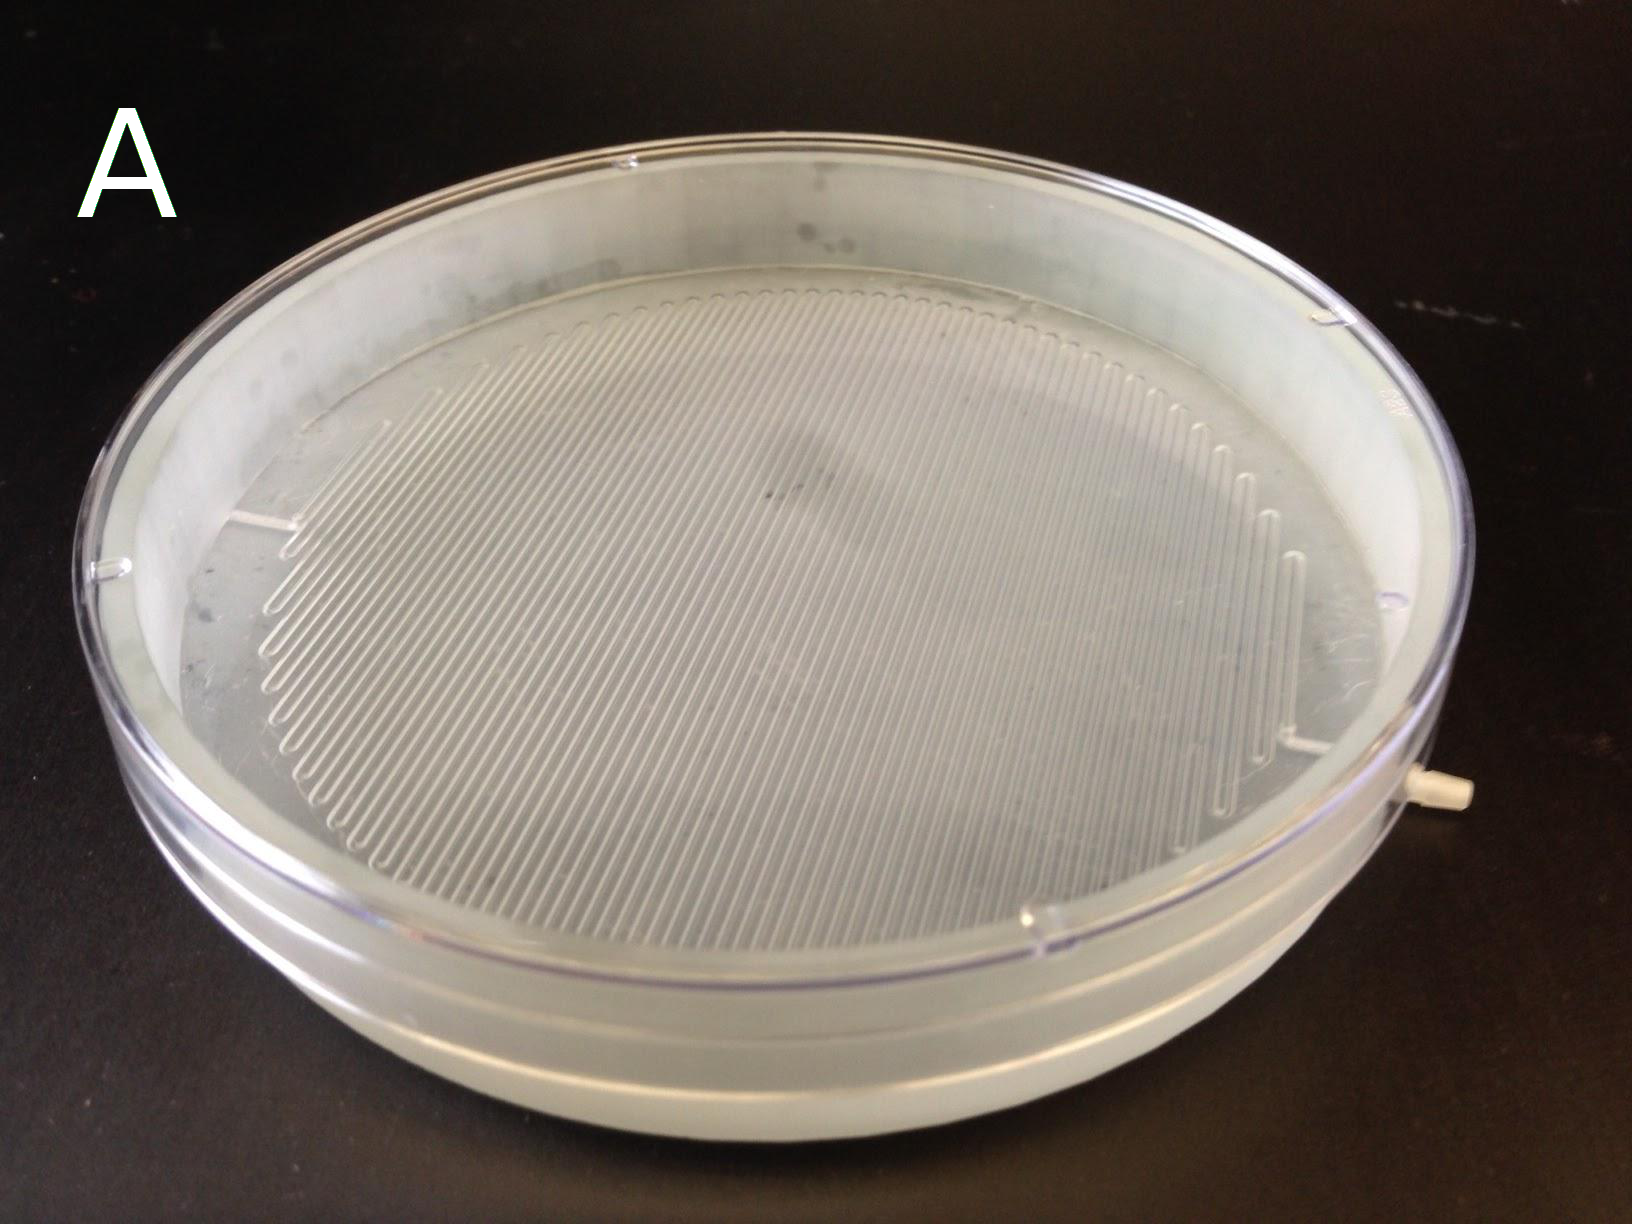
\includegraphics[scale=0.2]{3-inch-well-photo.png}
\caption{3" petri dish device}
\label{fig:3-inch-well-photo}
\end{figure}

\section{CONCLUSION}

3D printing allows complex designs, integrated tubing connectors, and is comparable in price to standard PDMS fabrication.
This technique represents a bridge to commercialization where robust devices can be more easily shared and disseminated.
While injection molding, hot embossing, or other industrial processes are cheaper when making hundreds to thousands of devices, it is not practical to make a injection mold when making tens to hundreds of devices.
In addition, PDMS fabrication would be too time consuming, expensive, and the failure rate would be unacceptable.
3D printing is a perfect solution to these device fabrication needs.

\bibliographystyle{plain}
\bibliography{references}
\end{document}
